\subsection{2D CNN model}
The initial condition for the 2D problem is a Gaussian function with a standard deviation of 0.1 and a mean of 0.5.
The initial condition can be seen in \autoref{fig:2D_gauss_initial_condition}.
\begin{figure}[H]
    \centering
    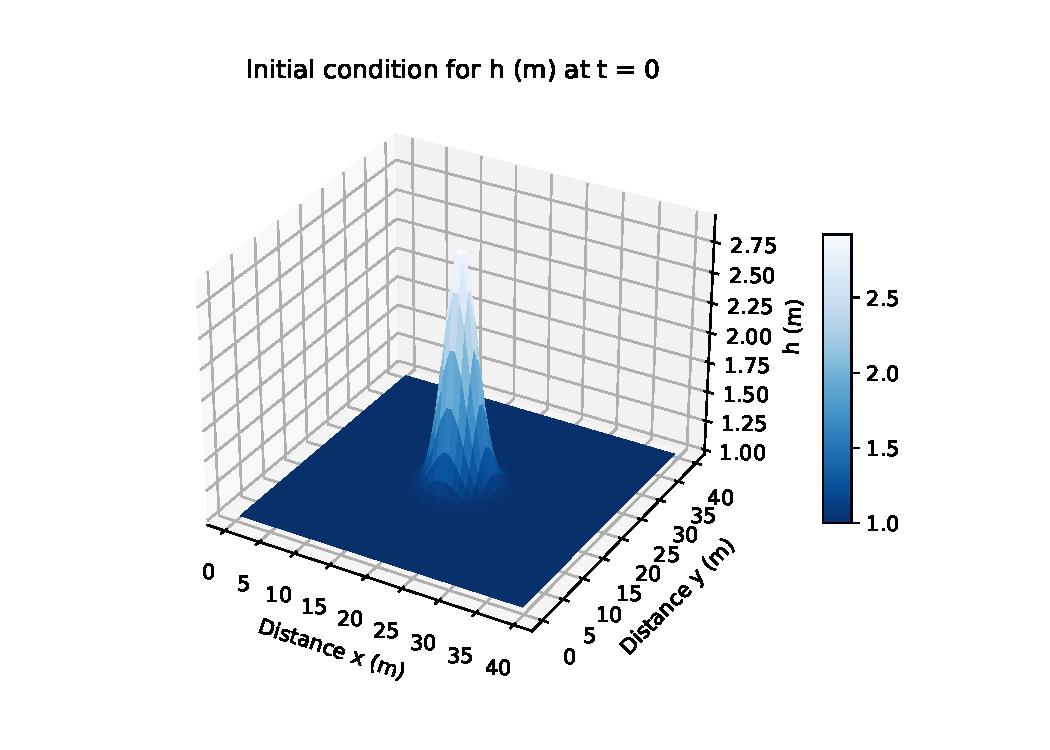
\includegraphics[width=0.8\textwidth]{C:/Users/Matteo/Shallow-Water-Equations/plots/2D_gauss_initial_condition.pdf}
    \caption{Initial condition for the 2D problem.}\label{fig:2D_gauss_initial_condition}
\end{figure}

The training and validation loss for the 2D CNN model can be seen in \autoref{fig:2D_CNN_loss}.
\begin{figure}[H]
    \centering
    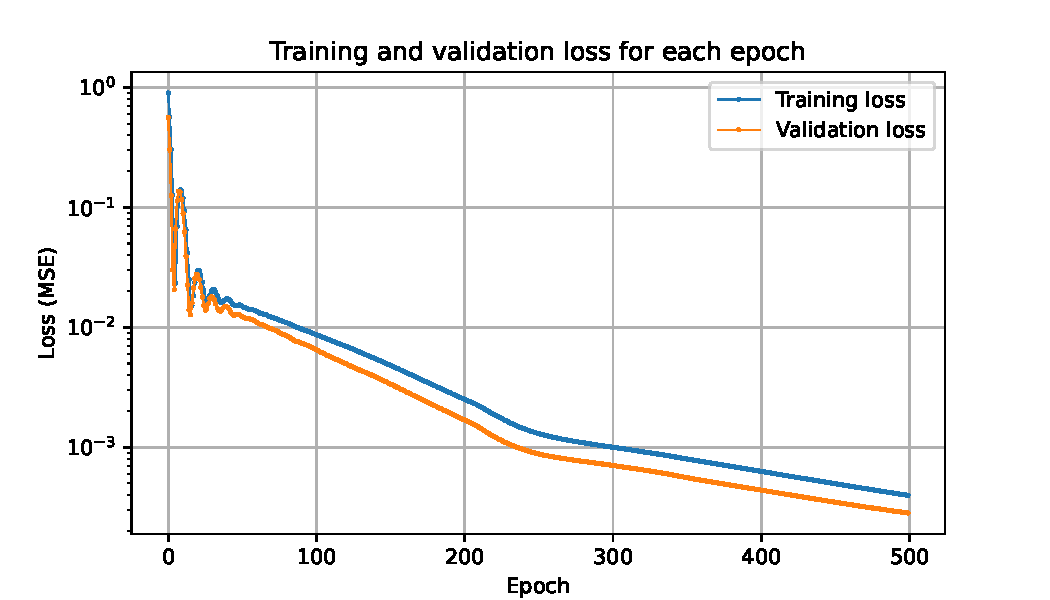
\includegraphics[width=0.7\textwidth]{C:/Users/Matteo/Shallow-Water-Equations/plots/2D_CNN_loss.pdf}
    \caption{Training and validation loss for the 2D CNN model.}\label{fig:2D_CNN_loss}
\end{figure}

The error plot for the last prediction for the 2D CNN can be seen in \autoref{fig:2D_CNN_error}.
\begin{figure}[H]
    \centering
    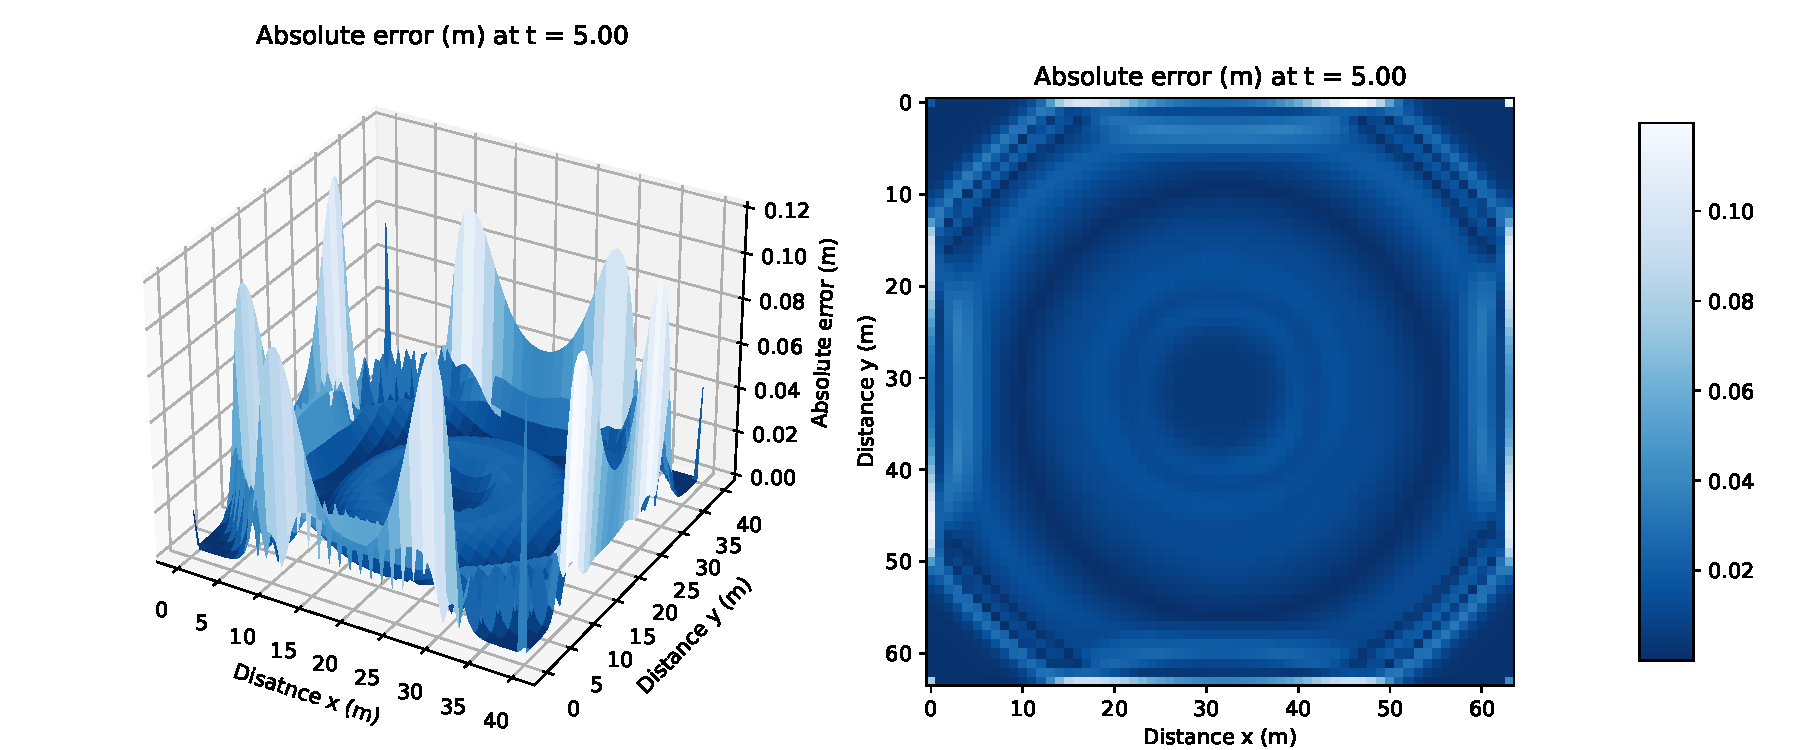
\includegraphics[width=0.8\textwidth]{C:/Users/Matteo/Shallow-Water-Equations/plots/2D_CNN_error.pdf}
    \caption{Error plot for the last prediction for the 2D CNN.}\label{fig:2D_CNN_error}
\end{figure}

\subsection{2D FNO Model}







